%
% Carátula NO-oficial para 86.22 aboratorio de Control Automático.
%
% Basado en el template realizado por Diego Essaya, disponible en
%                                                         http://lug.fi.uba.ar
% Modificado por Patricio Moreno y Michel Peterson.
% Modificado por Sebastián Santisi.
% Abril 2014: Modificado por Patricio Moreno.
% Septiembre 2017: Modificado por Patricio Moreno.
% Septiembre 2017: Modificado por Ezequiel Pecker Marcosig.

%
% Acá se define el tamaño de letra principal:
% Para utilizar los estilos de KOMA-script, descomentar la línea siguiente y
% comentar la que le sigue (dejar sin comentar un único documentclass)
%\documentclass[10pt]{scrartcl}
\documentclass[10pt]{article}

%
% Título y autor(es):
%
\title{Trabajo Práctico N\b o 1}
\author{CERVETTO, Marcos\\MARCHI, Edgardo\\PECKER MARCOSIG, Ezequiel}

%------------------------- Carga de paquetes ---------------------------
%
% Si no necesitás algún paquete, comentalo.
%

%
% Definición del tamaño de página y los márgenes:
% Si preferís menos márgenes, descomentá la línea anterior
%\usepackage[a4paper,headheight=16pt,scale={0.7,0.8},hoffset=0.5cm]{geometry}

%
% Vamos a escribir en castellano:
%
\usepackage[spanish,es-tabla]{babel}
\usepackage[utf8x]{inputenc}

%
% Para escribir fórmulas matemáticas utilizamos:
%
\usepackage{amsmath}
\usepackage{amssymb}
%
% El paquete amsmath agrega algunas funcionalidades extra a las fórmulas.
% Además defino la numeración de las tablas y figuras al estilo "Figura 2.3",
% en lugar de "Figura 7". (Por lo tanto, aunque no uses fórmulas, si querés
% este tipo de numeración dejá el paquete amsmath descomentado).
%
% \numberwithin{equation}{section}
% \numberwithin{figure}{section}
% \numberwithin{table}{section}

%
% Para tener cabecera y pie de página con un estilo personalizado:
%
\usepackage{fancyhdr}

%
% Para poner el texto "Figura X" en negrita:
% (Si no tenés el paquete 'caption2', probá con 'caption').
%
\usepackage[hang,bf]{caption2}

%
% Para poner hipervínculos en el pdf
%
\usepackage[colorlinks=true,linkcolor=black, urlcolor=blue]{hyperref}

%
% Para poder modificar los items de las listas (IEEE style refs.)
%
\usepackage{enumerate}

%
% Para poder usar subfiguras: (al estilo Figura 2.3(b) )
%
%\usepackage{subfig}

%
% Para poder armar tablas con formato
%
\usepackage{booktabs}

%
% Para poder agregar notas al pie en tablas:
%
%\usepackage{threeparttable}

%------------------------------ graphicx ----------------------------------
%
% Para incluir imágenes, el siguiente código carga el paquete graphicx
% según se esté generando un archivo dvi o un pdf (con pdflatex).

% Para generar dvi, descomentá la linea siguiente:
%\usepackage[dvips]{graphicx}

% Para generar pdf, descomentá las dos lineas seguientes:
\usepackage[pdftex]{graphicx}
\pdfcompresslevel=9

%
% Todas las imágenes están en el directorio imgs:
%
\newcommand{\imgdir}{imgs}
\graphicspath{{\imgdir/}}
%
%------------------------------ graphicx ----------------------------------

% Necesitas este paquete si haces los diagrámas de flujo en el prográma Dia
% y exportás a latex
%\usepackage{tikz}

%------------------------------ color -------------------------------------
% Necesitas este paquete para definir tus propios colores
\usepackage{color}
\definecolor{mygreen}{rgb}{0,0.6,0}
\definecolor{mygray}{rgb}{0.5,0.5,0.5}
\definecolor{mymauve}{rgb}{0.58,0,0.82}
%------------------------------ color -------------------------------------


%----------------------------- listings -----------------------------------
% Necesitas este paquete para mostrar el código.
\usepackage{listings}
\lstdefinestyle{customcpp}{
  backgroundcolor=\color{white},   % choose the background color; you must add \usepackage{color} or \usepackage{xcolor}; should come as last argument
  basicstyle=\small,        % the size of the fonts that are used for the code
  breakatwhitespace=false,         % sets if automatic breaks should only happen at whitespace
  breaklines=true,                 % sets automatic line breaking
  captionpos=b,                    % sets the caption-position to bottom
  commentstyle=\color{mygreen},    % comment style
  deletekeywords={...},            % if you want to delete keywords from the given language
%  escapeinside={\%*}{*)},          % if you want to add LaTeX within your code
  extendedchars=true,              % lets you use non-ASCII characters; for 8-bits encodings only, does not work with UTF-8
  frame=single,	                   % adds a frame around the code
  keepspaces=true,                 % keeps spaces in text, useful for keeping indentation of code (possibly needs columns=flexible)
  keywordstyle=\color{blue},       % keyword style
  language=C++,                 % the language of the code
  morekeywords={*,...},           % if you want to add more keywords to the set
%  numbers=left,                    % where to put the line-numbers; possible values are (none, left, right)
%  numbersep=5pt,                   % how far the line-numbers are from the code
%  numberstyle=\tiny\color{mygray}, % the style that is used for the line-numbers
  rulecolor=\color{black},         % if not set, the frame-color may be changed on line-breaks within not-black text (e.g. comments (green here))
  showspaces=false,                % show spaces everywhere adding particular underscores; it overrides 'showstringspaces'
  showstringspaces=false,          % underline spaces within strings only
  showtabs=false,                  % show tabs within strings adding particular underscores
  stepnumber=2,                    % the step between two line-numbers. If it's 1, each line will be numbered
  stringstyle=\color{mymauve},     % string literal style
  tabsize=2,	                   % sets default tabsize to 2 spaces
  title=\lstname                   % show the filename of files included with \lstinputlisting; also try caption instead of title
}

\lstdefinestyle{custommatlab}{
  backgroundcolor=\color{white},   % choose the background color; you must add \usepackage{color} or \usepackage{xcolor}; should come as last argument
  basicstyle=\small,        % the size of the fonts that are used for the code
  breakatwhitespace=false,         % sets if automatic breaks should only happen at whitespace
  breaklines=true,                 % sets automatic line breaking
  captionpos=b,                    % sets the caption-position to bottom
  commentstyle=\color{mygreen},    % comment style
  deletekeywords={...},            % if you want to delete keywords from the given language
%  escapeinside={\%*}{*)},          % if you want to add LaTeX within your code
  extendedchars=true,              % lets you use non-ASCII characters; for 8-bits encodings only, does not work with UTF-8
  frame=single,	                   % adds a frame around the code
  keepspaces=true,                 % keeps spaces in text, useful for keeping indentation of code (possibly needs columns=flexible)
  keywordstyle=\color{blue},       % keyword style
  language=Matlab,                 % the language of the code
  morekeywords={*,...},           % if you want to add more keywords to the set
%  numbers=left,                    % where to put the line-numbers; possible values are (none, left, right)
%  numbersep=5pt,                   % how far the line-numbers are from the code
%  numberstyle=\tiny\color{mygray}, % the style that is used for the line-numbers
  rulecolor=\color{black},         % if not set, the frame-color may be changed on line-breaks within not-black text (e.g. comments (green here))
  showspaces=false,                % show spaces everywhere adding particular underscores; it overrides 'showstringspaces'
  showstringspaces=false,          % underline spaces within strings only
  showtabs=false,                  % show tabs within strings adding particular underscores
  stepnumber=2,                    % the step between two line-numbers. If it's 1, each line will be numbered
  stringstyle=\color{mymauve},     % string literal style
  tabsize=2,	                   % sets default tabsize to 2 spaces
  title=\lstname                   % show the filename of files included with \lstinputlisting; also try caption instead of title
}
%----------------------------- listings -----------------------------------



%------------------------- Inicio del documento ---------------------------

\begin{document}

%
% Hago que en la cabecera de página se muestre a la derecha la sección,
% y en el pie, en número de página a la derecha:
%
\pagestyle{fancy}
\lhead{\sc TP Nº1 - \sc 2º Cuat. 2017}
\chead{}
\rhead{CERVETTO, MARCHI, PECKER MARCOSIG}
\lfoot{}
\cfoot{}
\rfoot{\thepage}

%
% Carátula:
%
\begin{titlepage}

\thispagestyle{empty}

\begin{center}

\includegraphics[scale=0.3]{img/fiuba}\\
\large{\textsc{Universidad de Buenos Aires}}\\
\large{\textsc{Facultad De Ciencias Exactas y Naturales}}\\
\large{\textsc{Departamento de Computación}}\\
% Modificar año y cuatrimestre
\small{Año 2017 - 2\textsuperscript{do} Cuatrimestre}
\end{center}

\vfill

\begin{center} % Modificar el código de ser necesario
\Large{\underline{\textsc{Simulación de Eventos Discretos}}}
\end{center}

\vfill

\begin{tabbing}
\hspace{2cm}\=\+TRABAJO PRÁCTICO Nº \textless{}1\textgreater{}\\
	TEMA:\textless{}Manejo del Inventario de una Industria\textgreater{}\\
	FECHA:\textless{\today}\textgreater{}\\
\\
	INTEGRANTES:\hspace{-1cm}\=\+\hspace{1cm}\=\hspace{6cm}\=\\
		CERVETTO, Marcos	\>\>- \#FIUBA\\
			\>\footnotesize{\verb!<cervettomarcos@gmail.com>!}\\
		MARCHI, Marcos	\>\>- \#FIUBA\\
			\>\footnotesize{\verb!<edgardo.marchi@gmail.com>!}\\
		PECKER MARCOSIG, Ezequiel	\>\>- \#FIUBA\\
			\>\footnotesize{\verb!<ezepecker@gmail.com>!}\\
\end{tabbing}

\vfill

\hrule
\vspace{0.2cm}

% Modificar código de ser necesario
\noindent\small{Simulación de Eventos Discretos}

\end{titlepage}

%
% Hago que las páginas se comiencen a contar a partir de aquí:
%
\setcounter{page}{1}

%
% Pongo el índice en una página aparte:
%
\tableofcontents
\newpage

%
% Inicio del TP:
%

\section{Enunciado}
Acá va el enunciado del trabajo, o al menos la parte relevante del problema
planteado.

Este documento tiene por objetivos: a) servir de plantilla para los informes 
de los Trabajos Prácticos de la materia Laboratorio de Control Automático 
con las secciones mínimas que deberían incluírse, y b) dar \textit{guías de estilo} 
para la elaboración de los mismos.

Se recomienda organizar el informe en secciones y subsecciones para facilitar el flujo de la información y su lectura. Las secciones y subsecciones del presente documento pretenden dar una idea de una posible organización pero no son exhaustivas.

%\flushleft\includegraphics[scale=0.75]{especificacion.pdf}


\section{Modelo Conceptual}
\subsection{Motivación}
Motivación
Una compañía que vende un único producto está interesada en estimar cuántas unidades del mismo debería tener en inventario en los próximos n meses (n es un parámetro de entrada fijo).

La compañía cuenta básicamente con tres proveedores de diferentes materias primas. Cada producto se fabrica usando 1 unidad de cada materia prima.

La planta está compuesta por un departamento de control de inventario, un departamento de atención al cliente y control de calidad de producto (ya que los productos son perecederos), un stock de productos finalizados y tres stocks de materias primas (uno para cada material). Las demandas de la clientela se producen aleatoriamente en pedidos de 1 a 4 unidades (también aleatorios). Existen 3 tipos diferentes de demanda.

En la Figura 1 se propone un esquema del proceso. Se puede observar que el top model consiste de tres jerarquías. En una jerarquía se encuentran: los tres proveedores, los tres clientes y la industria, en la otra se encuentran los tres stock de materia prima, el departamento de atención al cliente y control de calidad de producto, y el departamento de control de inventario, y en el último nivel dentro de Atención al Cliente y Control de Calidad se encuentran ambos departamentos. Cada cliente consiste de un modelo atómico distinto para representar tres comportamientos distintos. De la misma manera se utilizan tres modelos atómicos para modelizar cada tipo de proveedor. Por cada materia prima se tendrá un stock distinto, que al tener el mismo comportamiento se modelizará con un único modelo atómico. Finalmente, para los departamentos de control de calidad y control de inventario se utilizarán dos modelos atómicos. En resúmen, el modelo de la Figura~\ref{fig:fig1} se conforma de 2 jerarquías, una superior con 7 bloques y una inferior con 3 modelos atómicos.

\begin{figure}
\centering
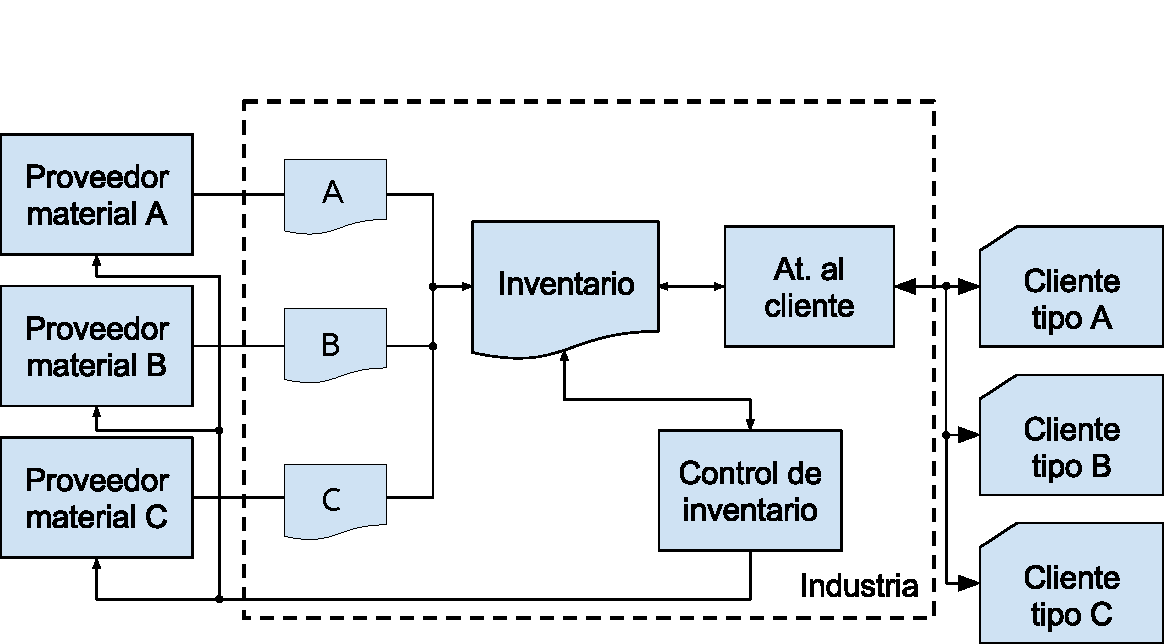
\includegraphics[scale=1]{img/figura1}
\caption{Esquema del problema planteado.}
\label{fig:fig1}
\end{figure}

La pregunta a responder mediante simulaciones es:
¿Qué política de reposición nos llevará a un manejo óptimo del nivel de stock logrando la mayor satisfacción del cliente y el menor costo de mantenimiento y reposición del inventario?
Una pregunta adicional que surge a partir de la anterior es ¿Cómo ponderar adecuadamente ambos requisitos en conflicto?

\subsection{Modelización}
A continuación en cada subsección se describe cada uno de los bloques de la Figura 1.

\subsubsection{Demanda (cliente)}
Los tiempos entre demandas por tipo de cliente son variables aleatorias exponenciales e independientemente distribuidas con una media de 0,12 mes. Los tamaños de las demandas (que pueden ir de uno a cuatro unidades del producto), D, son variables aleatorias independientemente distribuidas e independientes, cuya probabilidad de ocurrencia se muestra en la Tabla~\ref{tab:tabla1}.

\begin{table}[t]
\begin{center}
\begin{tabular}{cc}
\toprule
\textbf{D (\# Unidades)} & \textbf{Probabilidad}\\
\midrule
1 unidad & $1/6$\\
2 unidades & $1/3$\\
3 unidades & $1/3$\\
4 unidades & $1/6$\\
\bottomrule
\end{tabular}
\end{center}
\caption{Demanda.}
\label{tab:tabla1}
\end{table}

Existen 3 tipos de políticas de demanda: A, B y C. Un cliente tipo A encarga siempre $n$ productos y los retira a principio de mes. Un cliente tipo B pide $n$ productos pero se lleva solamente los que haya disponibles en stock en ese momento y los restantes para completar su pedido quedan encargados. Finalmente un cliente tipo C pide $n$ productos pero solamente compra si están disponibles, sino rechaza la compra.

El modelo que representa el comportamiento de los clientes tipo A se puede observar en la Figura~\ref{fig:fig2}, donde la salida \texttt{E\_OUT} indica la cantidad de productos encargados.

\begin{figure}
\centering
\includegraphics[scale=1]{img/figura2}
\caption{Modelo de cliente tipo A.}
\label{fig:fig2}
\end{figure}

El modelo utilizado para el comportamiento de los clientes de tipo B se muestra en la Figura~\ref{fig:fig3}. Las salidas \texttt{P\_OUT}, \texttt{E\_OUT} y \texttt{Q\_OUT} indican respectivamente la cantidad de productos retirados, la cantidad de productos encargados y la cantidad de productos pedidos.

\begin{figure}
\centering
\includegraphics[scale=1]{img/figura3}
\caption{Modelo de cliente tipo B.}
\label{fig:fig3}
\end{figure}

Finalmente, el modelo del comportamiento de los clientes de tipo C se muestra en la Figura~\ref{fig:fig4}.

\begin{figure}
\centering
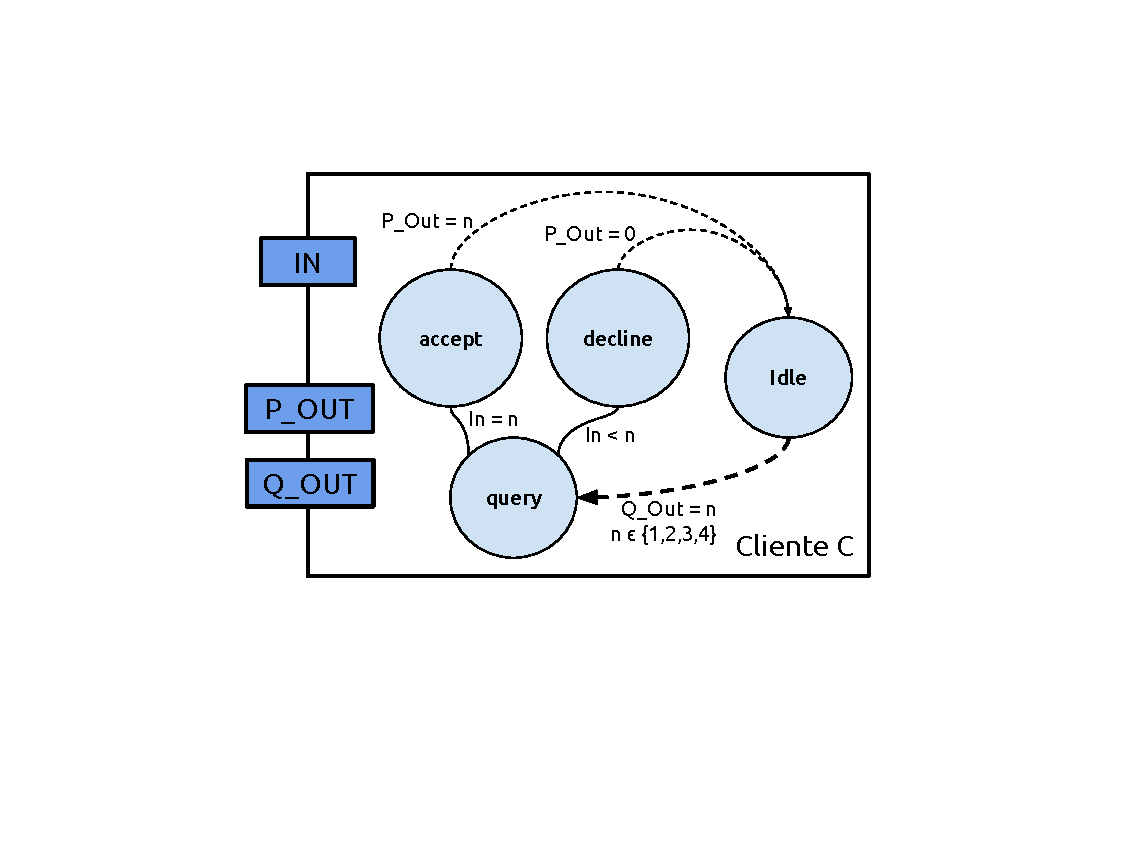
\includegraphics[scale=1]{img/figura4}
\caption{Modelo de cliente tipo C.}
\label{fig:fig4}
\end{figure}

\subsubsection{Atención al cliente y control de calidad}
En la Figura~\ref{fig:fig5} se puede observar el comportamiento del módulo acoplado de Atención al Cliente y Control de Calidad. El departamento de Control de Calidad se encarga de examinar los productos al momento de venta y verificar su fecha de vencimiento. Los insumos con los que se elabora el producto son perecederos, y su vida útil está uniformemente distribuida entre 1,5 y 2,5 meses. Por tanto, la fecha de vencimiento del producto se determina como el mínimo entre las fechas de vencimiento de los insumos con los que se elaboró. La compañía descubre que una unidad no sirve más solamente cuando la examina debido a una venta. Si una unidad no sirve más, se desecha  y se examina la siguiente unidad existente en el inventario. Se computan también las proporciones de unidades que se descartan.

\begin{figure}
\centering
\includegraphics[scale=1]{img/figura5}
\caption{Atención al cliente.}
\label{fig:fig5}
\end{figure}

\subsubsection{Control de inventario}

Al comienzo de cada mes, la compañía revisa el nivel de inventario y decide cuántas nuevas unidades pedir a sus proveedores. La compañía ordena $Z$ unidades a todos los proveedores por igual. El costo costo será $K + pZ$, donde $K = 350~\textrm{pesos}$ es el costo fijo del pedido y $p = 25~\textrm{pesos}$ es el costo incremental por unidad. Naturalmente, si $Z = 0$ no se incurre en ningún costo. La compañía usa la siguiente política para decidir cuántas unidades pedir: si $I$ es el nivel de inventario al comienzo del mes, $S$ el inventario máximo posible (capacidad de almacenamiento) y $s$ el parámetro de política de reposición, $Z$ estará dado por:

\begin{equation}
Z=\left\{\begin{array}{lr}
		S – I & \textrm{si}\qquad I < s\\
		0 & \textrm{si} \qquad I \geq s
	\end{array}\right.
\label{eq:ctrlinv}
\end{equation}

El modelo está dado por la Figura~\ref{fig:fig6}, donde se observa que hay tres estados: Query, Calc y Wait.

\begin{figure}
\centering
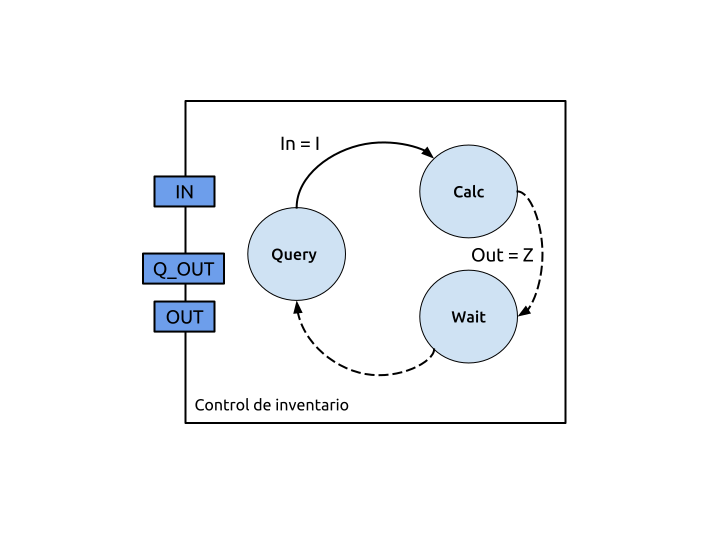
\includegraphics[scale=1]{img/figura6}
\caption{Esquema del control de inventario.}
\label{fig:fig6}
\end{figure}


\subsubsection{Inventario}

Ante una consulta de un cliente el inventario responde con la cantidad de unidades disponibles en ese momento. En base a esto y a la política de cada cliente, al inventario se le pide una cantidad determinada de unidades para retiro y/ó encargue.
El inventario lleva una lista de unidades disponibles y una de unidades encargadas. Cuando una reposición llega, se usa primero para eliminar todos los pedidos pendientes (si hay) posibles; el resto de la reposición (si queda) se suma al inventario. 

\begin{figure}
\centering
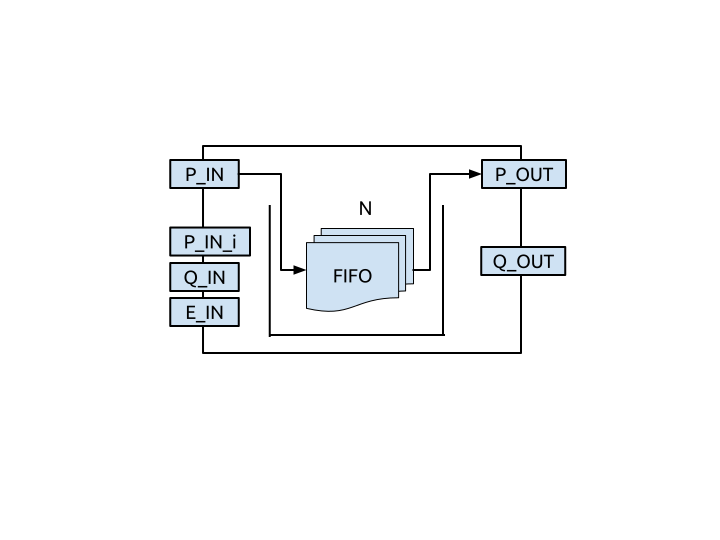
\includegraphics[scale=1]{img/figura7}
\caption{Inventario.}
\label{fig:fig7}
\end{figure}

%En la Figura~\ref{fig:fig7} se observa el modelo con que se representa al Inventario. El mismo consiste de una cola FIFO (\textit{first in - first out}). Se denomina $N$ al largo de la cola.
Suponemos también que la compañía incurre en un costo de mantenimiento del producto $h = 8~\textrm{pesos}$ por unidad por mes mantenido en inventario (positivo). Este costo incluye alquiler del depósito de almacenamiento, seguro, impuestos y mantenimiento, al igual que costo de oportunidad de tener capital inmobilizado en inventario en vez de invertido en otra parte. Supongamos además que hay un costo de \textit{demanda insatisfecha} $n = 50~\textrm{pesos}$ por unidad pedida por cliente y no suministrada y por mes. Este costo contabiliza tanto el costo de mantener registros adicionales para unidades ya asignadas a clientes y aún no suministradas como un cálculo de costo por pérdida de la buena voluntad del cliente.


\subsubsection{Proveedores}

Los proveedores se comportan de 3 formas diferentes: 
\begin{enumerate}[i)]
\item inmediato.
\item por múltiplo de cantidad fija.
\item por encargo.
\end{enumerate}

\begin{enumerate}[i)]
\item Al hacer un pedido al proveedor inmediato de $n$ unidades, entrega las $n$ unidades en forma instantánea. Las $n$ unidades asociadas tienen un tiempo de vencimiento asociado (Figura~\ref{fig:fig8}).

\begin{figure}
\centering
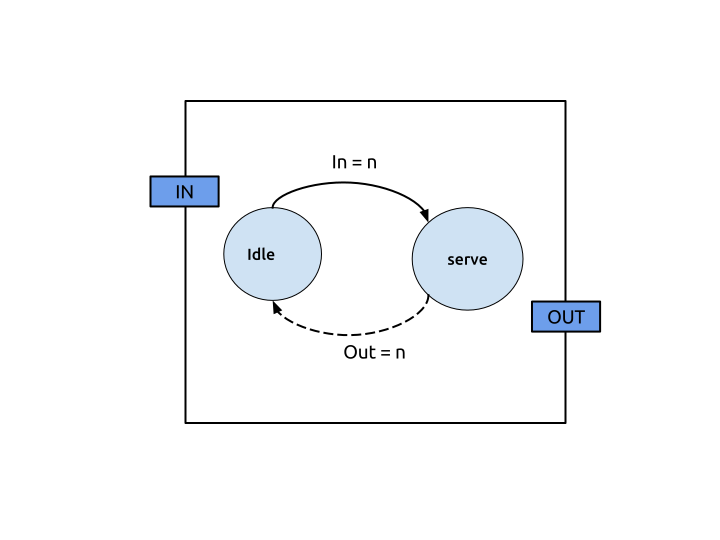
\includegraphics[scale=1]{img/figura8}
\caption{Proveedor $1$.}
\label{fig:fig8}
\end{figure}

\item El proveedor que funciona por múltiplo de cantidad fija, sólo entrega pedidos múltiplos de un número entero prefijado, digamos r (Figura~\ref{fig:fig9}). Es decir, que al hacer un pedido de n productos, pueden pasar 2 cosas:

\begin{enumerate}[1)]
\item El número pedido $n$ equivale a un múltiplo entero de $r$, $n = k r$, para algún $k \geq 0$, en cuyo caso se entregan exactamente $n$ unidades.
\item El número pedido $n$ es mayor a un múltiplo entero de $r$, es decir, $n > k r$ y además $n < (k+1)r$, para algún $k \geq 0$, en cuyo caso se entregan $(k+1)r$ unidades.
\end{enumerate}

Los productos de este proveedor no tienen vencimiento.

\begin{figure}
\centering
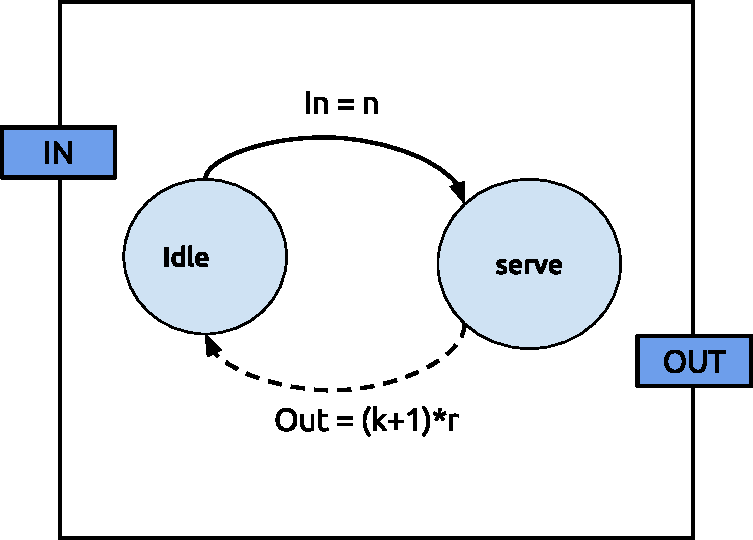
\includegraphics[scale=1]{img/figura9}
\caption{Proveedor $2$.}
\label{fig:fig9}
\end{figure}

\item El tercer proveedor (Figura~\ref{fig:fig10}) funciona por encargo para el mes siguiente. Es decir, todo pedido será servido en el siguiente mes. En ese momento, además, se realizará el nuevo pedido.

\begin{figure}
\centering
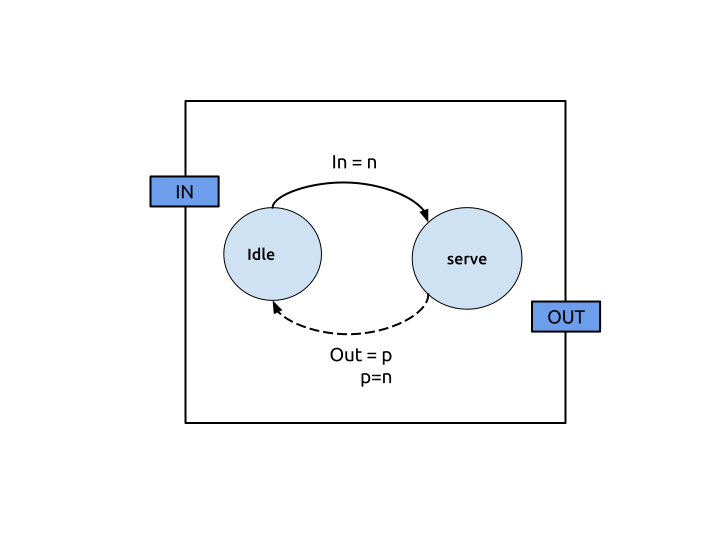
\includegraphics[scale=1]{img/figura10}
\caption{Proveedor $3$.}
\label{fig:fig10}
\end{figure}
\end{enumerate}

\section{Descripción Formal}
\subsection{Tipo de Cliente A}

En la Figura~\ref{fig:pdftiempo} y Figura~\ref{fig:pdfpedidos} se observan los histogramas que representan a la tasa de arribos de pedidos de clientes de tipo A y a la cantidad de unidades pedidas. El eje de tiempos de la Figura~\ref{fig:pdftiempo} se utiliza en segundos en lugar de en meses.

\begin{figure}
\centering
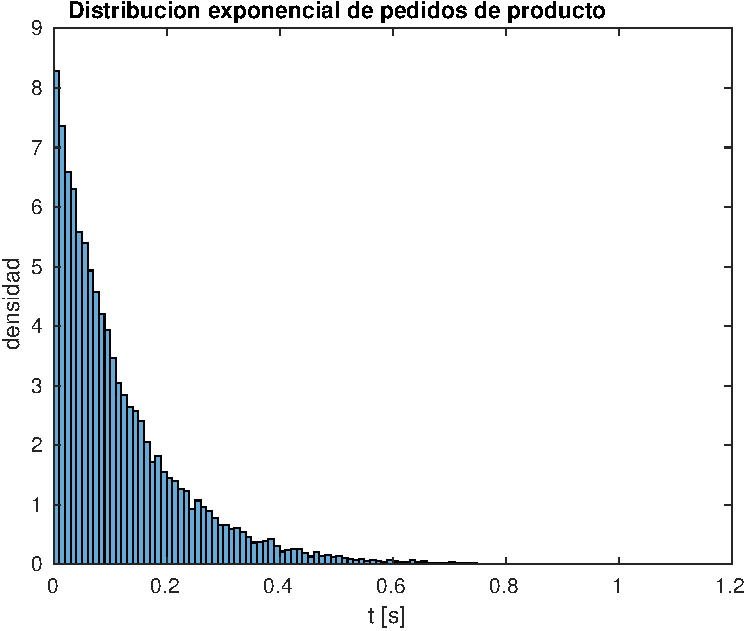
\includegraphics[scale=1]{img/pdf_tiempo_pedidos}
\caption{Función de densidad de probabilidad del tiempo entre pedidos de clientes tipo A.}
\label{fig:pdftiempo}
\end{figure}

\begin{figure}
\centering
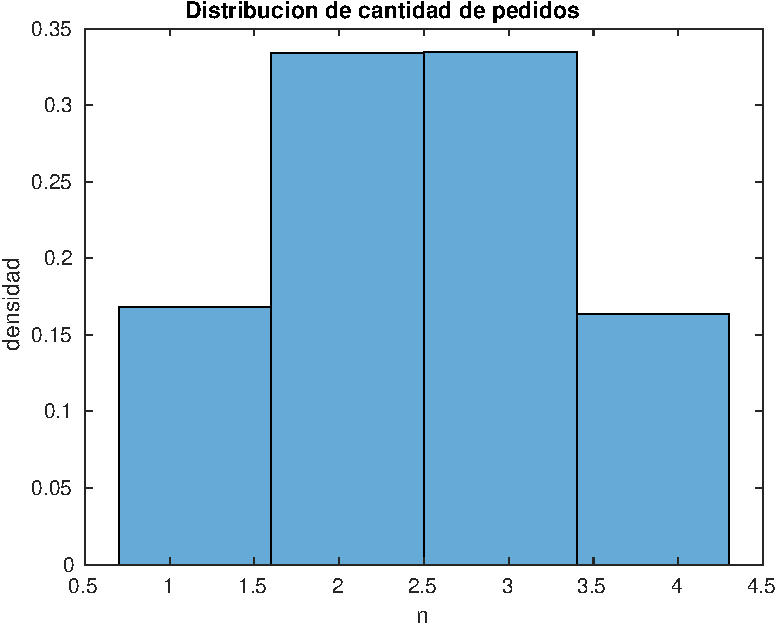
\includegraphics[scale=1]{img/pdf_cantidad_pedidos}
\caption{Función de densidad de probabilidad del número de unidades pedidas $n$.}
\label{fig:pdfpedidos}
\end{figure}

\begin{footnotesize}
\begin{minipage}{\textwidth}
  %\hspace{-1.4cm}
  \framebox[1\textwidth]{
  \begin{minipage}[t]{0.45\textwidth}
    $S:$ \hspace*{1mm} $\left\{\mathbf{phase},\mathbf{sigma},\mathbf{clienteA}\right\}$\\
    $X:$ \hspace*{1mm} $\left\{\emptyset\right\}$\\
    $Y:$ \hspace*{1mm} $\left\{n \in \left\{1,2,3,4\right\}\right\}$\\
    $\delta_{int}(s):$ 
    \hspace*{1mm} sigma = exp\_var($\mu$) \textbf{// Internal Transition} \\
    $\delta_{ext}(s,e,x):$  \textbf{// External Transition}
  \end{minipage}\hspace*{0.05\textwidth}
  \begin{minipage}[t]{0.45\textwidth}
    $\lambda(s):$
    \hspace*{5mm} query\_o = \textbf{eval}(discrete\_var) \textbf{// Output} \\
    $ta(s):$ \hspace*{4mm} \textbf{return} sigma \textbf{// Time advance}
  \end{minipage}}
\end{minipage}
\end{footnotesize}

\subsection{Tipo de Cliente B}
\subsection{Tipo de Cliente C}

\subsection{Control de inventario}
El modelo atómico correspondiente al bloque de control de inventario queda definido de la siguiente manera:


\framebox[1\textwidth]{
\begin{minipage}{0.9\textwidth}
	$CI=<S,X,Y,\delta_{int},\delta_{ext},\lambda,t_A>$\\
	
	$S=\{WAITING, QUERY, CALC\}$\\
	
	$X=\{numProd\_i\} \in \mathbb{N}^+_0 $\\
	
	$Y=\{queryInventory\_o, querySuppliers\_o\} \in \mathbb{N}^+_0$\\
	
	$\delta_{int}: \delta_{int}(S) \begin{cases}
		\delta_{int}(WAITING)=QUERY\\
		\delta_{int}(CALC)=WAITING
		\end{cases}$\\
		
	$\delta_{ext}:\delta_{ext}(S,numProd\_i) \begin{cases} Si ~S=QUERY \wedge  numProd\_i=N\\
	\hfill \rightarrow \delta_{ext}(S,numProd\_i)=CALC \end{cases}$\\
	
	$\lambda:~\lambda(S)\begin{cases}
	\lambda(WAITING)={queryInventory\_o = 1}\\
	\lambda(CALC)={querySuppliers\_o = \begin{cases}
		S-N~si~numProd\_i < s\\
		0~\forall~numProd\_i
		\end{cases}}
	\end{cases}$\\
	
	$t_A=\begin{cases}
	1~si~S=WAITING\\
	0~si~S=CALC\\
	\infty~si~S=QUERY
	\end{cases}$
\end{minipage}
}

En las figuras \ref{fig:CI-esquematico} y \ref{fig:CI-estados} se pueden observar los puertos de entrada/salida y el diagrama de estados respectivamente.

\begin{figure}
	\centering
	
\includegraphics{img/fiuba}
	\caption{Entradas y salidas del modelo control de inventario}
	\label{fig:CI-esquematico}
\end{figure}

\begin{figure}
	\centering
	
\includegraphics{img/fiuba}
	\caption{Diagrama de estados para el modelo de control de inventario.}
	\label{fig:CI-estados}
\end{figure}


\section{Modelado y simulación}
\subsection{Pruebas parciales}
\subsubsection{Control de Inventario}
Para la purueba del bloque de control de inventario se propuso el siguiente estímulo:

\begin{minipage}{0.5\textwidth}
	\centering
	\begin{lstlisting}
	00:00:01:10 invLevel 8
	00:00:02:10 invLevel 190
	00:00:03:10 invLevel 49
	\end{lstlisting}

	\caption{Archivo "ev" de estímulo para el modelo de control de inventario}
\end{minipage}

\subsection{Pruebas de integración}
.
\subsection{Reporte y conclusiones}


\appendix
\section{Código Implementado}

% Please don't exchange the bibliographystyle style
\bibliographystyle{IEEEtran.bst}
% AUTHOR: Include your bib file here
\bibliography{IEEEexample}

\end{document}

